\documentclass[a4paper,11pt]{article}

\title{Solutions to unfolding distributions}
\author{ACM}
\date{\today}


\usepackage[english]{babel}
%FloatBarrier
\usepackage{placeins}
%H
\usepackage{float}
\usepackage{amsmath,amssymb,amsfonts}
\usepackage{graphicx}
\usepackage{amsmath}
\usepackage[pdftex,hyperfootnotes=false,pdfpagelabels,pagebackref]{hyperref}

% to make a analitical index/glossaries
%\usepackage[acronym,xindy,nonumberlist]{glossaries}
\usepackage[acronym,nonumberlist]{glossaries}
%\usepackage{makeidx}
\makeglossaries
%\makeindex

\usepackage{booktabs}

%caption
%\usepackage[font=small,format=plain,labelfont=bf,margin=0.05\columnwidth]{caption}
\usepackage[font=small,format=plain,labelfont=bf,margin=0.05\columnwidth]{caption}


%%%% DEFINE COMMANDS %%%%%%%%%%%
\newcommand{\meas} {\ensuremath \vec{y}}
\newcommand{\truth}{\ensuremath \vec{x}_\textup{T}}
\newcommand{\resp} {\ensuremath \mathbf{R}}
\newcommand{\back} {\ensuremath \vec{b}}

\newcommand{\respt}{\ensuremath \mathbf{\tilde{R}}}
\newcommand{\strength}{\ensuremath \vec{\mu} } 

\newcommand{\mc}{\ensuremath \vec{x}_\textup{MC}}
%% I version
\newcommand{\truthI}[1]{\ensuremath x^\textup{T}_{#1}}
\newcommand{\strengthI}[1]{\ensuremath \mu_{#1} }
\newcommand{\mcI}[1]{\ensuremath x^\textup{MC}_{#1}}
\newcommand{\respI}[2]{\ensuremath R_{#1,#2} }
\newcommand{\resptI}[2]{\ensuremath \tilde{R}_{#1,#2} }

%% FIG 
\newcommand{\Left}{\mbox{(Left)}}
\newcommand{\Right}{\mbox{(Right)}}

%%%  Draft
\newcommand{\fixme}[1]{ \mbox{\bf{FIXME:} \it{#1}} } 


\newacronym{MC}{MC}{Monte Carlo}
\newacronym{BLUE}{BLUE}{best linear unbiased estimator}
\newacronym{ML}{ML}{maximum likelihood}
\newacronym{SVD}{SVD}{singular value decomposition}



\begin{document}
\maketitle

\section{Understanding unfolding}

The Unfolded spectra can be found using, eg, RooUnfold:
\begin{verbatim}
ROOT.gSystem.Load("${HOME}/Downloads/RooUnfold-1.1.1/libRooUnfold.so")
##  prepare the response matrix
# assume a flat prior
R = ROOT.RooUnfoldResponse(None,None,resp)
u = ROOT.RooUnfoldInvert(R,reco)
u.SetName("unfolder1")
h = u.Hreco(ROOT.RooUnfold.kNone) 
h.SetName("unfold")

## for meaningful errors
fluct=1.0
for j in range(0,reco.GetNbinsX() ):
	reco_fluct.SetBinError(j+1,fluct)

u2 = ROOT.RooUnfoldInvert(R,reco_fluct)
u2.SetName("unfolder2")
u2.SetNToys(1000)
h2 = u2.Hreco( ROOT.RooUnfold.kCovToy) ##  error propagation down with toys
h2.SetName("unfold2")

\end{verbatim}

The result is shown in figure~\ref{fig:sol1}: the unfolded distribution with no-fluctuations should be by-construction identical to the one used for generating it; 
small differences may be due to the numeric precision of the floating point representation inside a computer, that act as a fluctuation smearing. 
The one that had fluctuations inside, nevertheless is the \gls{ML} estimator and therefore the \gls{BLUE}, has a very huge variance.

\begin{figure}[H]
	\centering
	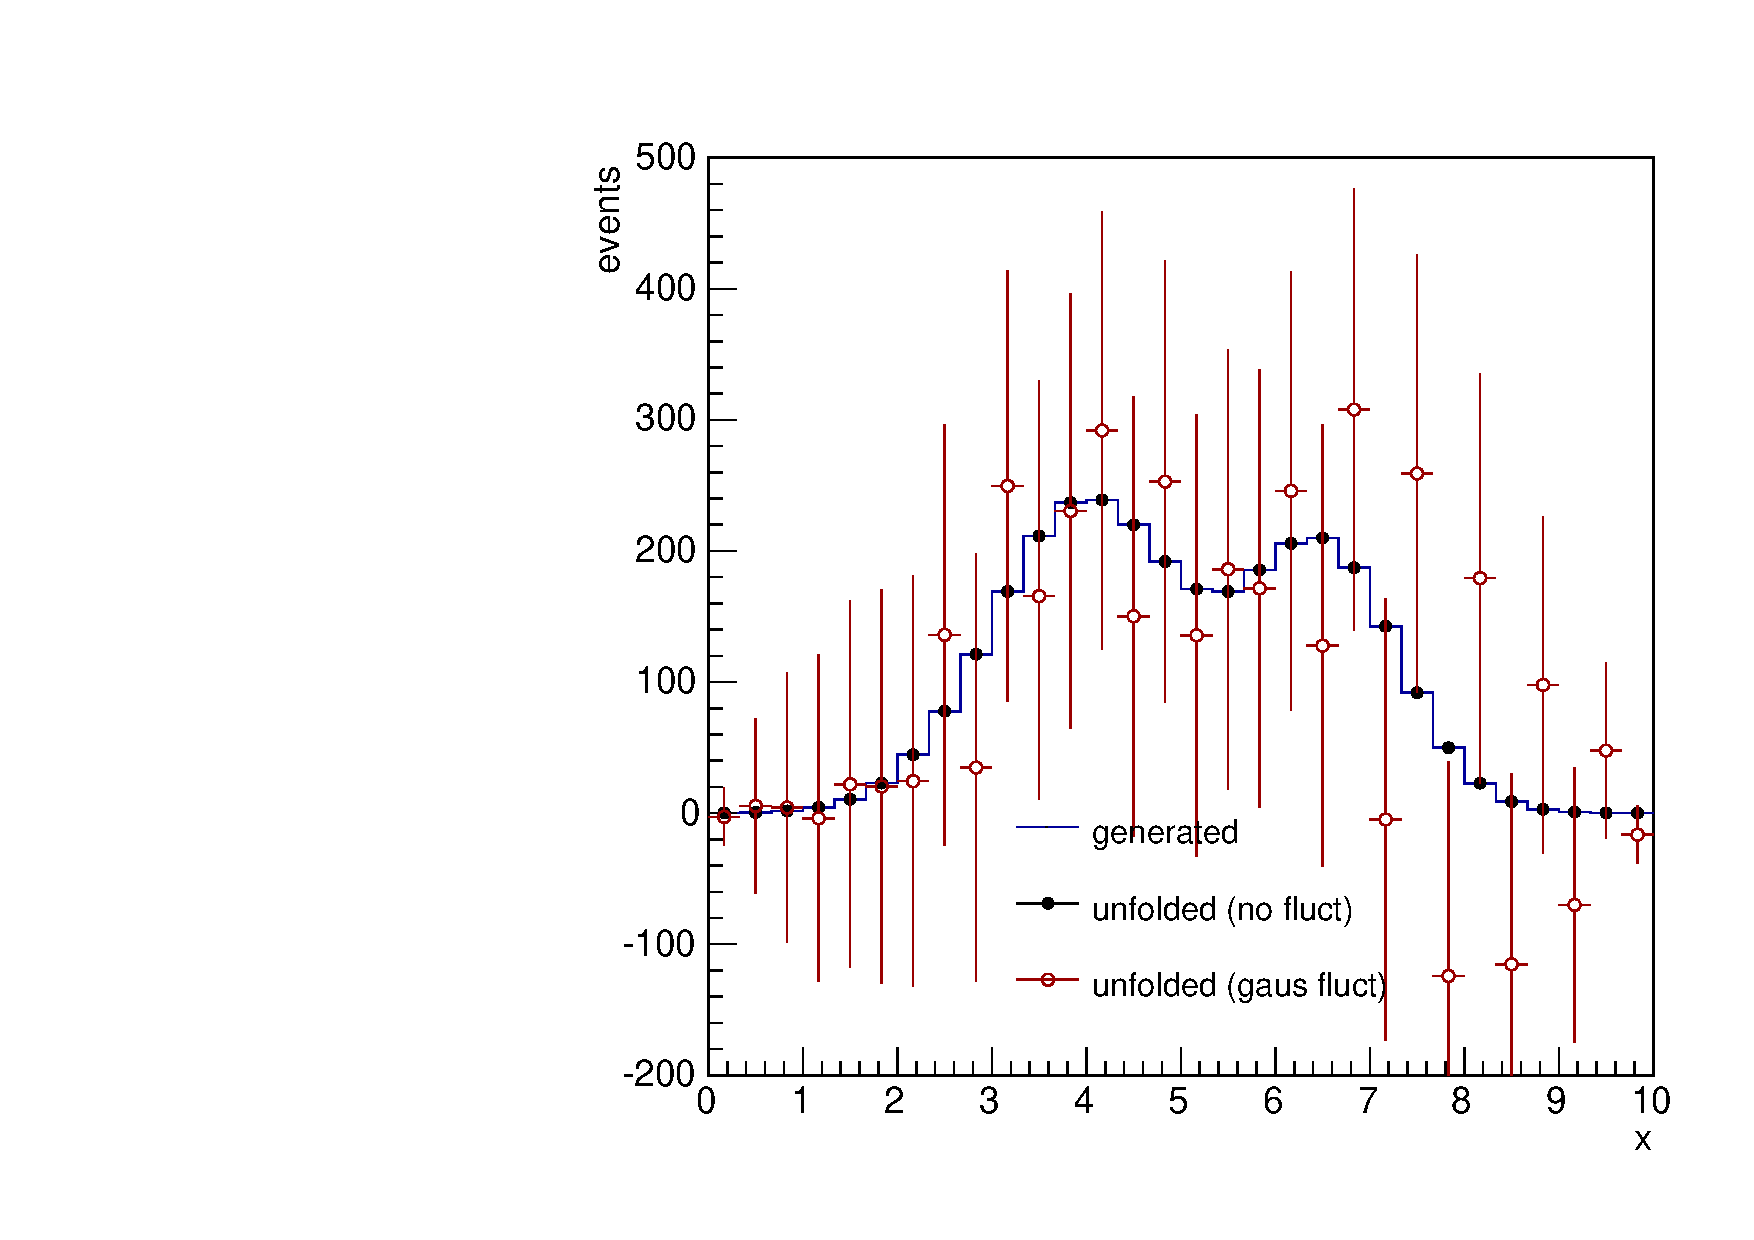
\includegraphics[width=0.618\textwidth]{figs/gen-unfold.pdf}
	\caption{ \label{fig:sol1} The two unfolded distribution compared with the one used to generate them.}
\end{figure}

\FloatBarrier
\section{Regularization}
Regularization techniques are used to cure the high variance of the distribution, introducing an ad hoc bias. 

We start studying regularization to see the effect that it has on the distributions:
\begin{figure}[H]
	\centering
	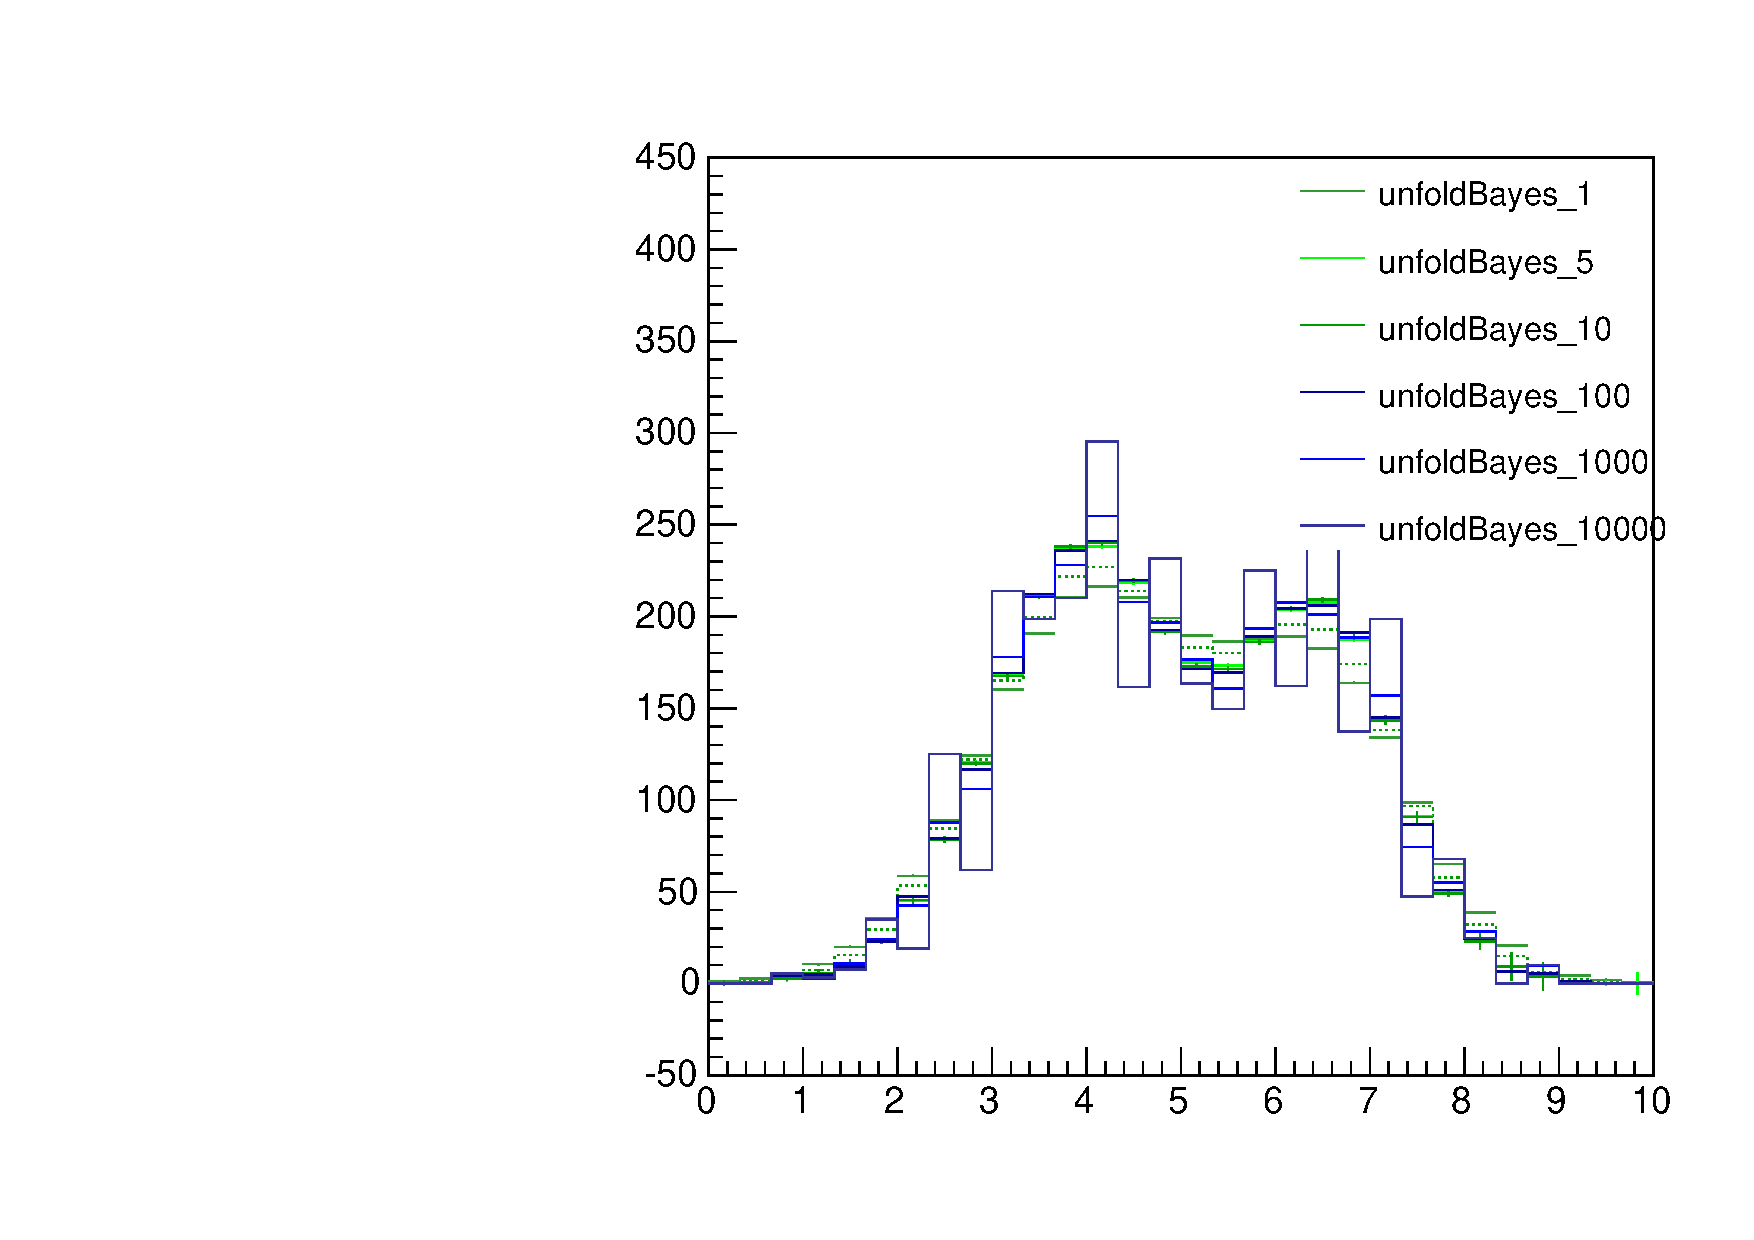
\includegraphics[width=0.49\textwidth]{figs/unfold-bayes-reg.pdf}
	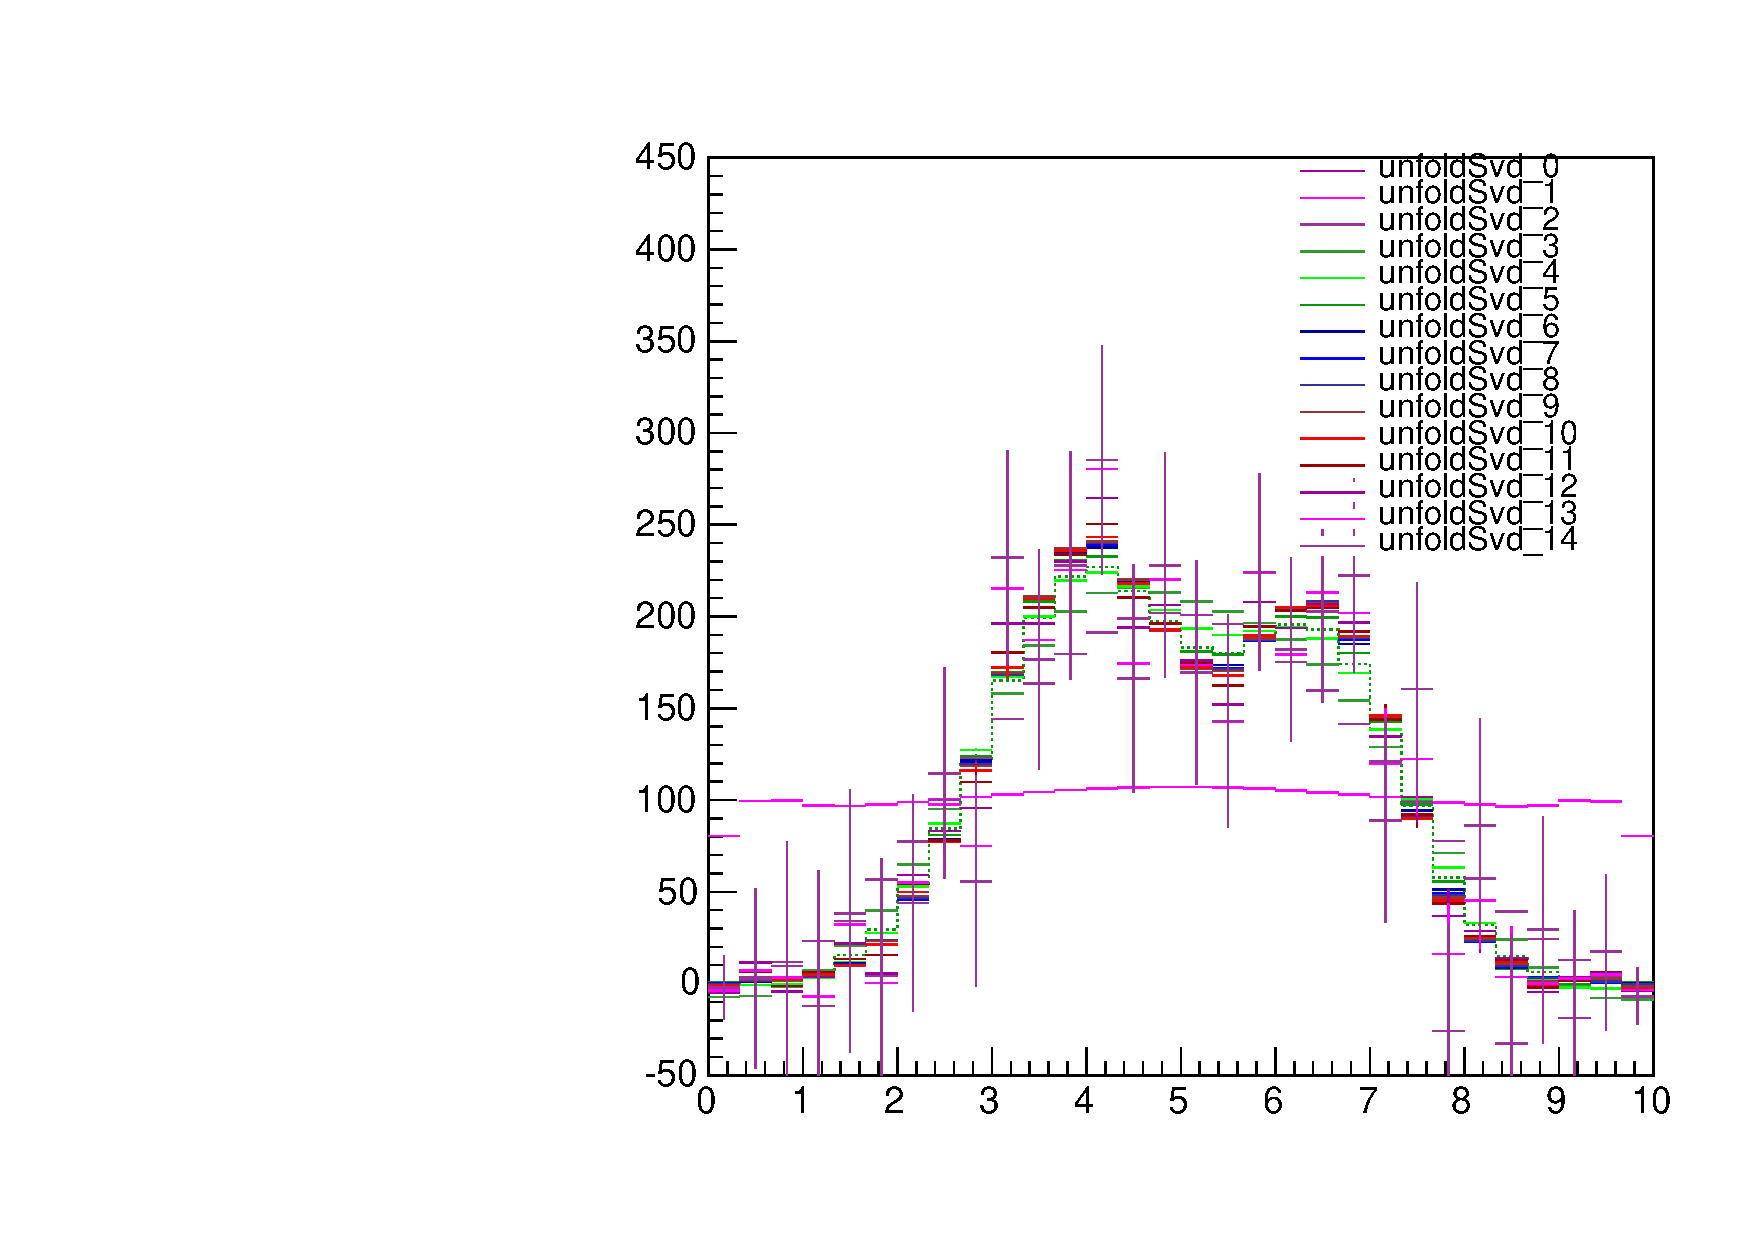
\includegraphics[width=0.49\textwidth]{figs/unfold-svd-reg.pdf}
	\caption{ \label{fig:sol:reg} The unfolded distribution for different regularization parameters. On the left, the iterative unfolding, on the right the Tickonov regularization. }
\end{figure}

For the iterative method based on Bayes' theorem the regularization is given by the number of iteration; the less iterations the closer the unfolded distribution to the prior we choose, usually obtained from \gls{MC}. The method will converge to the \gls{ML} solution with the increasing number of iterations.
For the \gls{SVD} implementation of the Tikonov regularization, the regularization is given by the number of singular values used in the inversion. The less singular values, the more the distribution is regularized. Using ``all'' the singular values we get close the \gls{ML} solution.

The regularization parameter is a \emph{choice} to make. 
There is no right and wrong value, but some wanted features are:
\begin{itemize}
	\item stability of the regularization with respect to the chosen regularization parameter.
	\item for the \gls{SVD}-method look at the $d_i$ distribution; in this case it shows that after $~10$ the distribution is random.
	\item error estimation after the unfolding should not be smaller than the one before it.
	\item use different predictions (if available) to evaluate possible biases.
\end{itemize}

\begin{figure}[H]
	\centering
	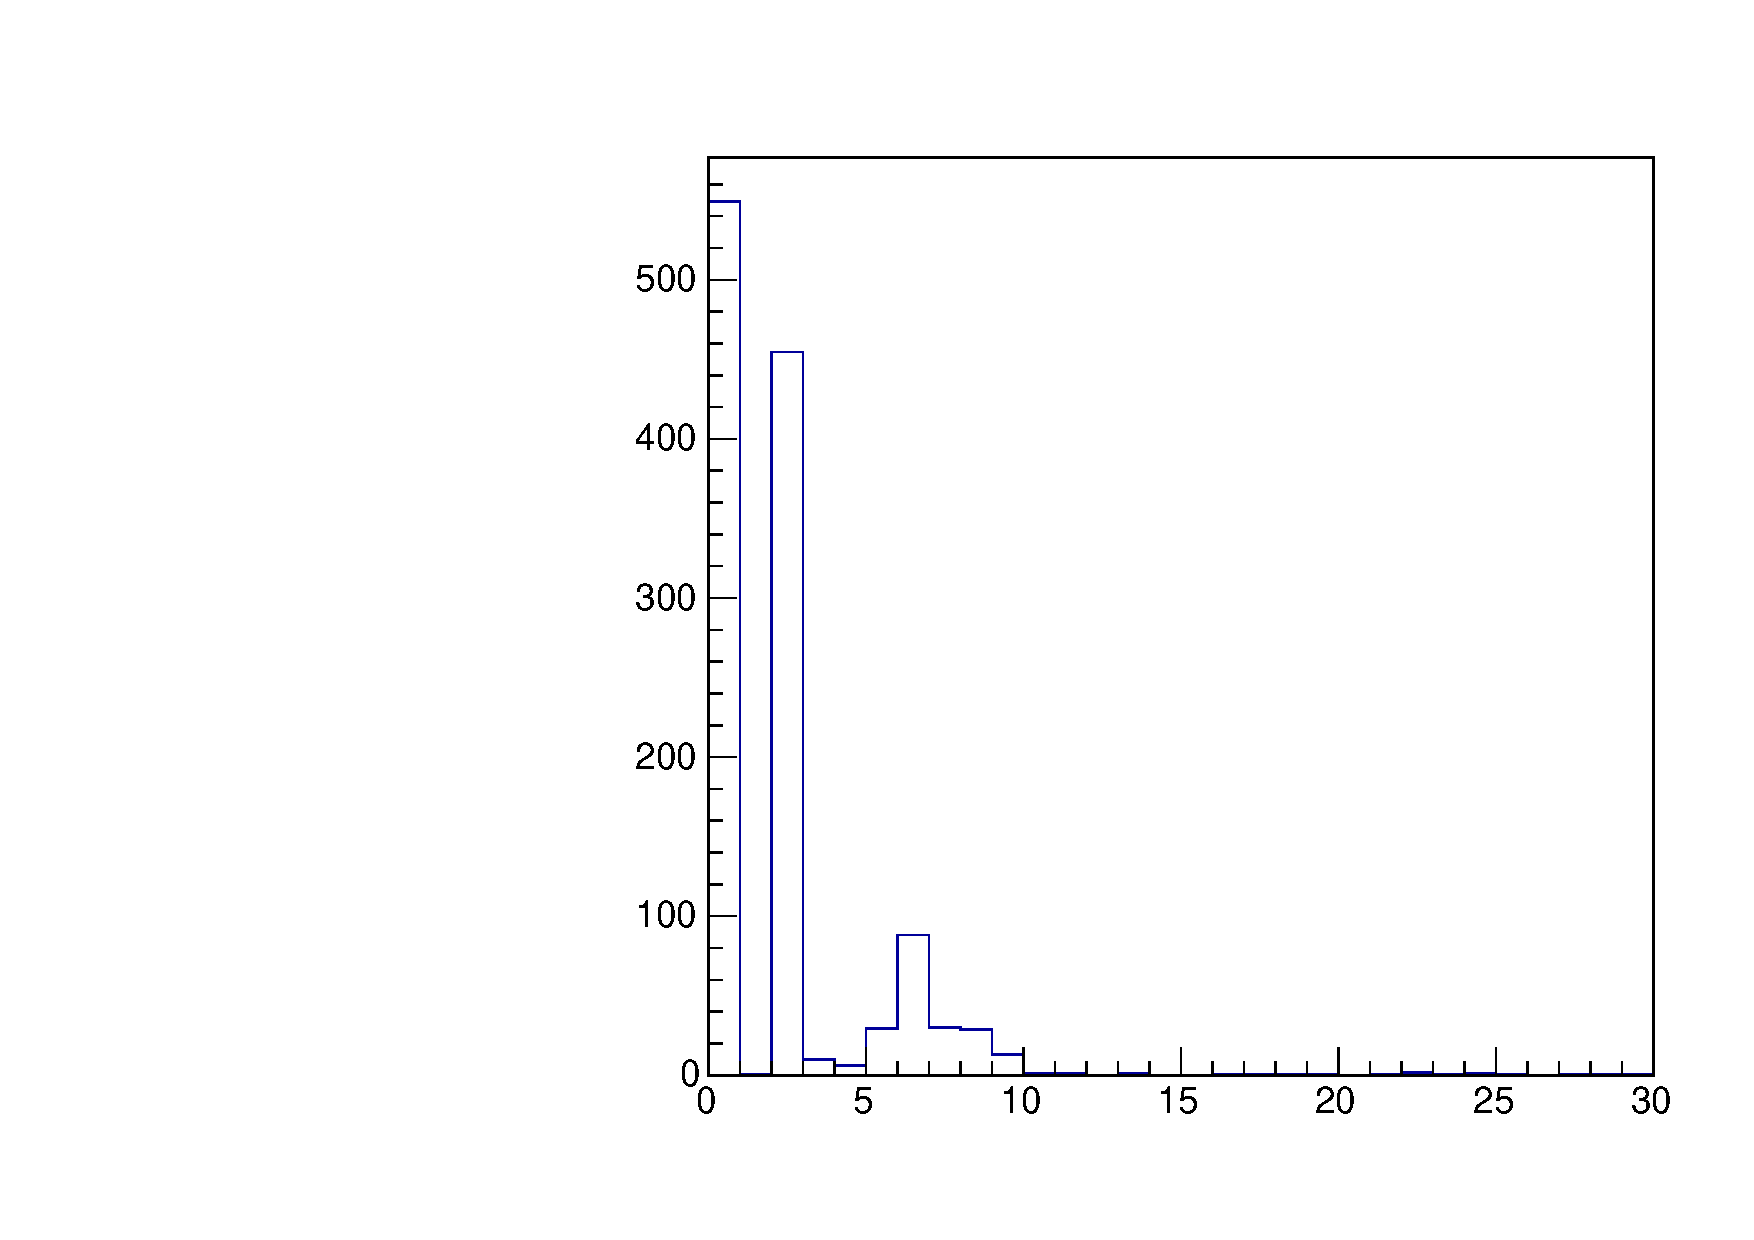
\includegraphics[width=0.49\textwidth]{figs/unfold-svd-ddistr.pdf}
	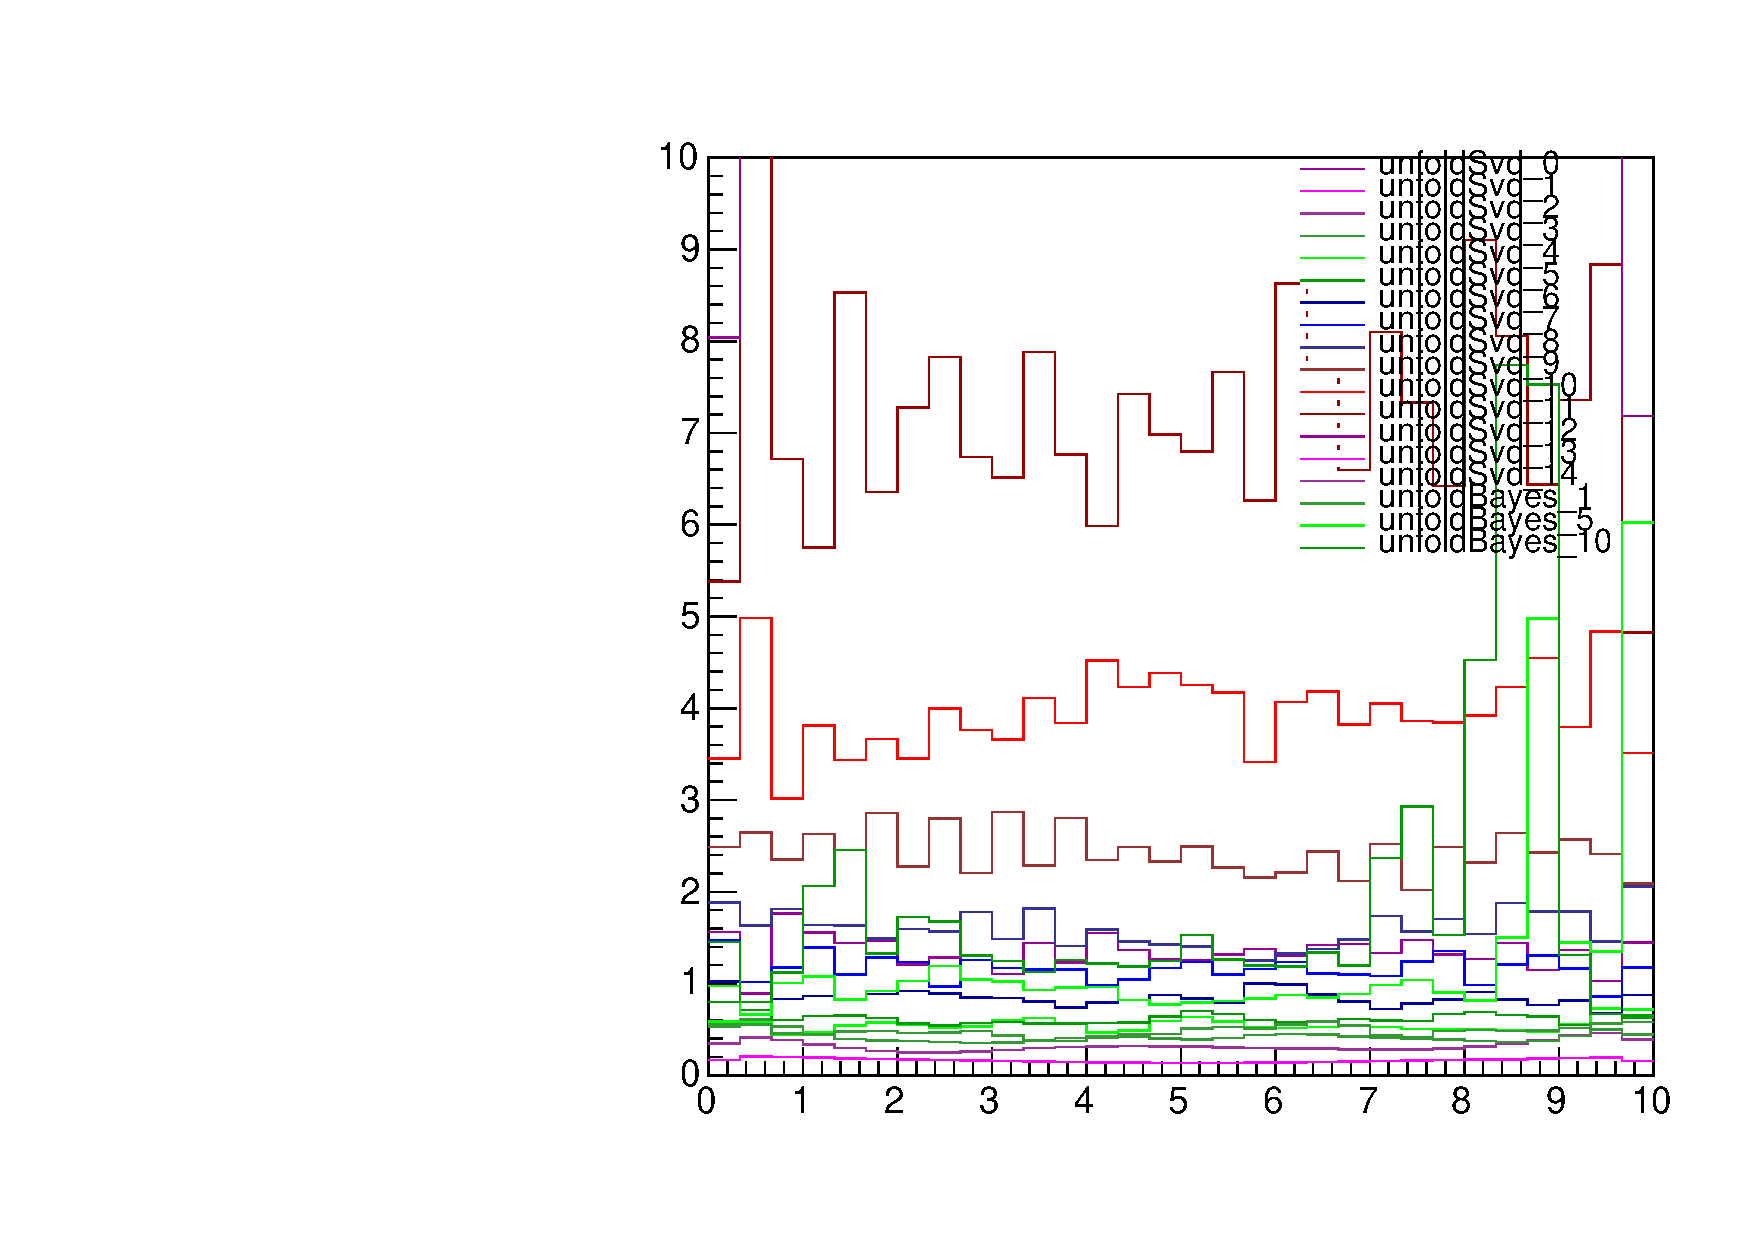
\includegraphics[width=0.49\textwidth]{figs/unfold-error-reg.pdf}
	\caption{ \label{fig:sol:reg2} Left: $d_i$-distribution for the \gls{SVD}-method. Right: ratio of the error before and after the unfolding.}
\end{figure}

\FloatBarrier
\section{Construct the response matrix}

The response matrix can be constructed in the following steps:

1)  Define a flag to identify if the event is in the fiducial region at the measured/truth level:
\begin{verbatim}
        isGen = t.lep1PtTruth >=15 and t.lep2PtTruth >= 15 \  
                and abs(t.lep1EtaTruth )<2.5 and abs(t.lep2EtaTruth) <2.5
        isReco = t.lep1PtReco >=15 and t.lep2PtReco >= 15  
                and abs(t.lep1EtaReco )<2.5 and abs(t.lep2EtaReco) <2.5
\end{verbatim}

2) Compute the scale factor as product of the two lepton scale factors.

3) Fill the gen histogram if is generated:
\begin{verbatim}
        if isGen: hTruth.Fill(Z.Pt(), t.weight ) # no sf
\end{verbatim}

4) Fill the reconstructed level with the scale factors
\begin{verbatim}
        if isReco: hReco.Fill( LL.Pt(), t.weight * mysf)
\end{verbatim}

5) Fill the smearing matrix iff both level are matched:
\begin{verbatim}
        if isGen and isReco:hMatrix.Fill(LL.Pt(),Z.Pt(),t.weight*mysf)
\end{verbatim}


6) Unfold the distribution, eg:
\begin{verbatim}
        R = ROOT.RooUnfoldResponse(hReco,hTruth,hMatrix)
        u = ROOT.RooUnfoldBayes(R,hData,5)
\end{verbatim}

Results can be seen in figure~\ref{fig:sol:exe2}, along of a couple of poissible mistakes.

\begin{figure}[H]
	\centering 
	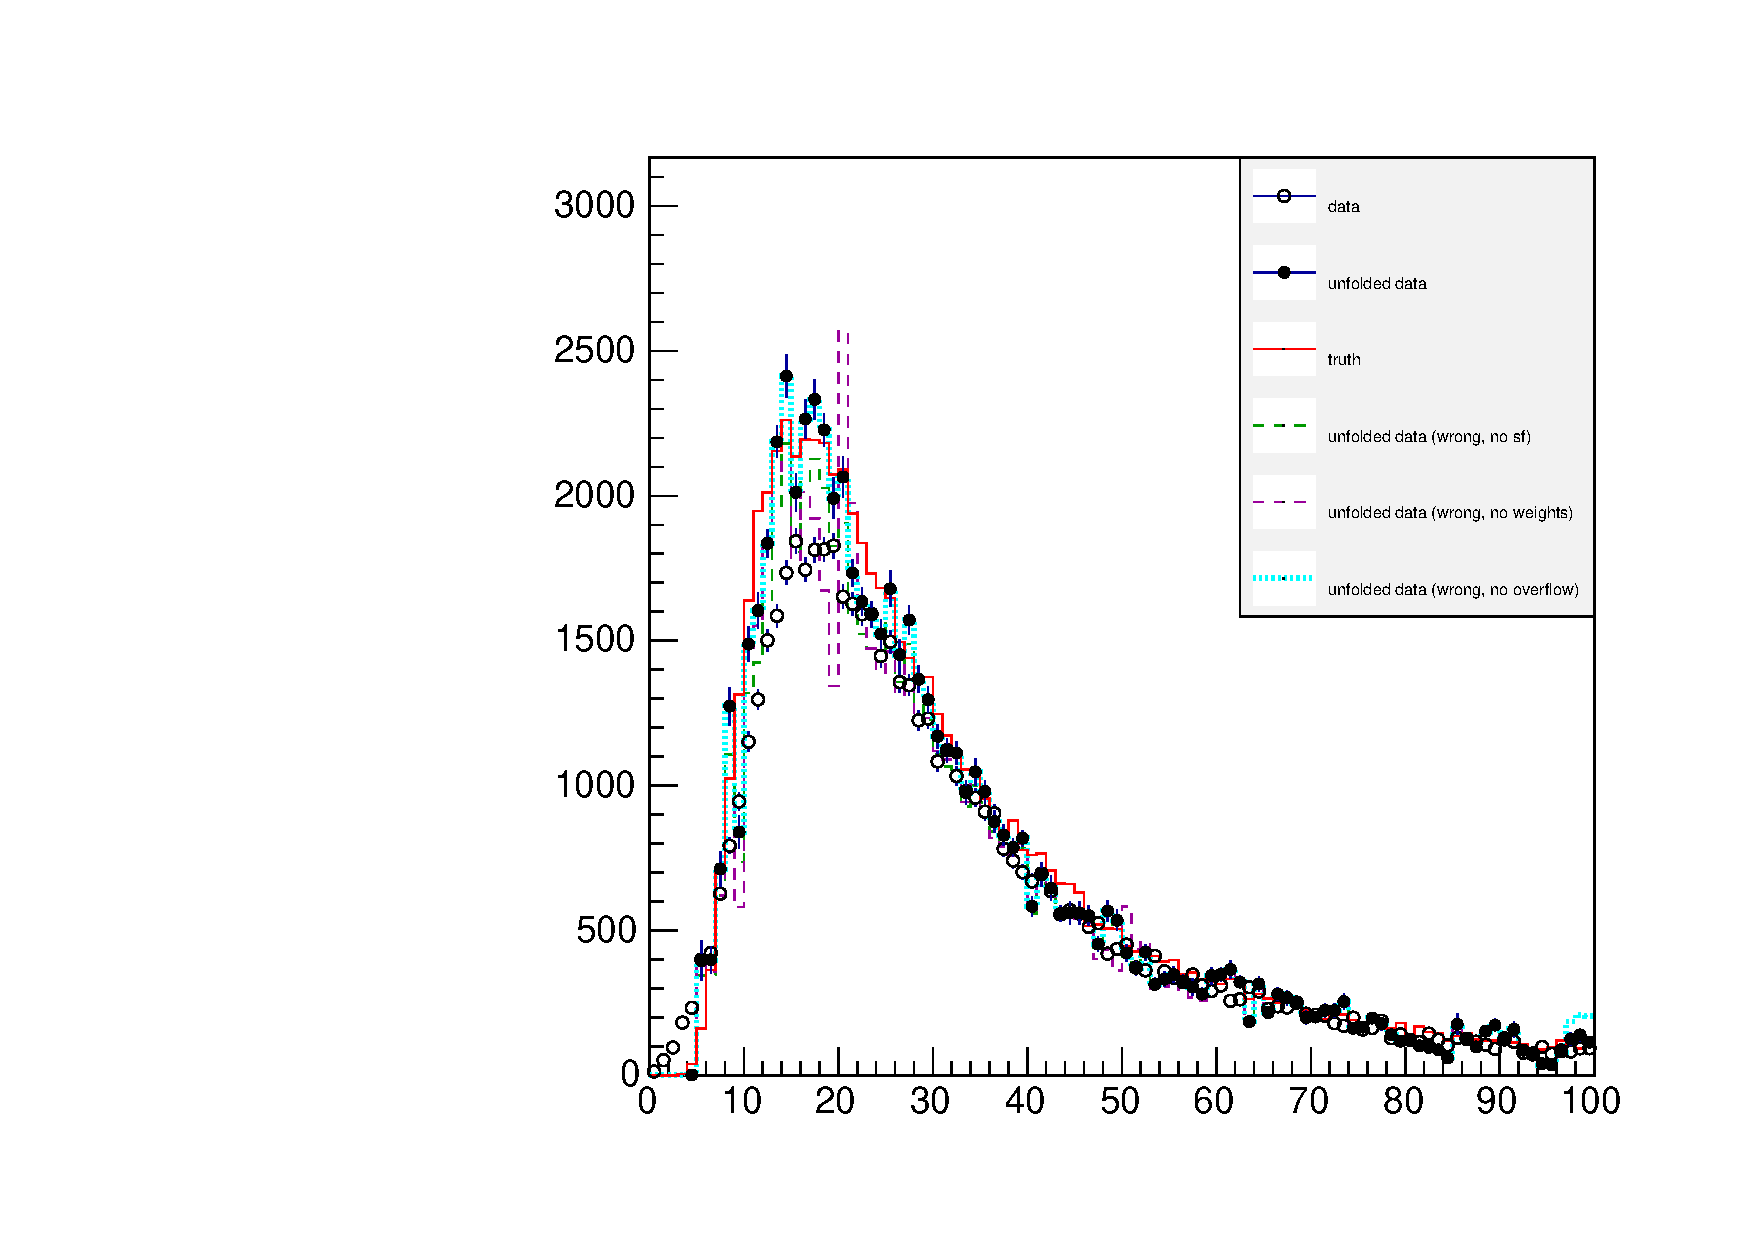
\includegraphics[width=.95\textwidth]{figs2/unfolding2.pdf}
	\caption{ \label{fig:sol:exe2} Unfolded distribution (solid black dots) compared to the reconstructed data distribution (empty dots). Underlying can be seen the distribution used to generate the data, prior poisson fluctuations (red), and two examples of wrongly unfolded distributions (dashed): the first without applying scale-factors (green), the second considering no weights at all (magenta).
	}
\end{figure}

\end{document}
